\section{Zielsetzung}
\label{sec:Zielsetzung}
In diesem Versuch wird die Suszeptibilität stark paramagnetischer Materialien 
mithilfe einer Brückenschaltung untersucht. 
\nocite{anleitungV606}

\section{Theorie}
\label{sec:Theorie}
In Materie wird die magnetische Flussdichte $\vec{B}$ durch die magnetische Feldstärke
$\vec{H}$, die Induktionskonstante $\mu _0$ und die Magnetisierung $\vec{M}$ wie folgt beschrieben
\begin{equation}
    \vec{B} = \mu _0 \vec{H} + \vec{M}\,.
    \label{eqn:magnetischeFlussdichte}
\end{equation}
Dabei hängt $\vec{M}$ mit $\vec{H}$ durch 
\begin{equation}
    \vec{M} = \mu _0\, \chi\, \vec{H}
    \label{eqn:Magnetisierung}
\end{equation}
zusammen. Hierbei beschreibt $\chi$ die Suszeptibilität, welche keine Konstante ist, sondern von $\vec{H}$ und der Temperatur $T$ abhängt.
Der Diamagnetismus tritt für alle Atome auf, weil durch ein von außen angelegtes Magnetfeld ein magnetischer Moment induziert wird. Dadurch
entsteht ein induziertes Magnetfeld, was dem äußeren Magnetfeld entgegengerichtet ist. Daher gilt beim Diamagnetimus für die Suszeptibilität
$\chi < 0 $. Anders als beim Diamagnetismus, tritt der Paramagnetismus nur bei Atomen, Ionen oder Molekülen mit einem nicht veschwindenen Drehimpuls auf.
Dieser entsteht durch die relativ zum äußeren Magnetfeld ausgerichteten magnetischen Momente, die mit dem Drehimpuls gekoppelt sind. Zusätzlich ist der
Paramagnetismus im Vergleich zum Diamagnetimus temperaturabhängig, da die Ausrichtung der magnischten Moment durch
die thermische Bewegung gestört wird. Bei einem nicht zu starken äußeren Magnetfeld auf die Atome gilt für den Gesamtdrehimpuls $\vec{J}$
\begin{equation}
    \vec{J} = \vec{L} + \vec{S}\,.
    \label{eqn:Gesamtdrehimpuls}
\end{equation}
Diese Gleichung wird ebenfalls als LS-Kopplung bezeichnet, wobei $\vec{L} = \sum_{i}{\vec{l}_{\text{i}}}$ den Gesamtbahndrehimpuls und 
$\vec{S} = \sum_{i}{\vec{s}_{\text{i}}}$ den Gesamtspin beschreibt.
Die zugehörigen magnetischen Momente zu dem Drehimpuls $\vec{L}$ und dem Spin $\vec{S}$ lauten
\begin{align}
    \vec{\mu _{\text{L}}} &= - \frac{\mu_{\text{B}}}{\hbar}\,\vec{L}\quad\text{und} \label{eqn:magnetischerMommentDrehimpuls} \\
    \vec{\mu _ {\text{S}}} &= -g_{\text{S}}\frac{\mu_{\text{B}}}{\hbar}\,\vec{S}\,. \label{eqn:magnetischerMomentSpin}
\end{align}
$\hbar$ ist das reduzierte Planksche Wirkungsquantum, $g_{\text{S}}$ ist das gyromagnetische Verhältnis des freien Elektrons und 
\begin{equation}
    \mu _{\text{B}} = \frac{1}{2} \frac{e_0}{m_0}\,\hbar
    \label{eqn:BohrscheMagneton}
\end{equation}
ist das Bohrsche Magneton, wobei $e_0$ die Ladung und $m_0$ die Ruhemasse des Elektrons sind. 
In der Quantenmechanik wird $g_{\text{S}} \approx 2$ genähert, wodurch mit dem Landé-Faktor
\begin{equation}
    g_{\text{L}} = \frac{3\,J \left(J+1\right) + \big(S\left(S +1\right) -L\left(L+1\right)\big)}{2\,J\left(J+1\right)} 
    \label{eqn:LandeFaktor}
\end{equation}
für den Betrag des magnetischen Moments 
\begin{equation}
    \left|\vec{\mu_{\text{J}}}\right| \approx \mu_{\text{B}}\,g_{\text{J}}\sqrt{J\left(J+1\right)}
    \label{eqn:magnetischerMoment}
\end{equation}
gilt. Daraus folgt für die potentielle Energie mit der Orientierungsquantenzahl $m$
\begin{equation}
    E_{\text{m}} = \mu_{\text{B}}\,g_{\text{J}}\, m\, B\,. 
    \label{eqn:E_pot}
\end{equation}
Ein Zeeman-Effekt tritt dann auf wenn die durch die Gleichung (\ref{eqn:E_pot}) beschriebene Aufspaltung eines Energieniveaus
in $2J+1$ Unterniveaus beim Anlegen eines Feldes an eine Probe mit permanenten magnetischen Momenten stattfindet.
Die Verteilung der magnetischen Momente ist durch die Boltzmann-Verteilung gegeben. Die Magnetisierung wird mithilfe dem mittleren magnetischen 
Moment und der Brillouin-Funktion bestimmt. Daraus folgt aus einer Näherung von schwachen Feldern und der Raumtemperatur für die Magnetisierung
\begin{equation}
    M = \frac{1}{3}\mu _0\,\mu_{\text{B}}^2\,g_{\text{B}}^2\,N \frac{J(J+1)B}{kT}\,.
    \label{eqn:Magnetisierung_Naeherung}
\end{equation}
Demnach ergibt sich für die paramagnetische Suszeptibilität 
\begin{equation}
    \chi = \frac{1}{3}\mu _0\,\mu_{\text{B}}^2\,g_{\text{B}}^2\,N \frac{J(J+1)}{kT}\,,
    \label{eqn:paramagnetische_Suszeptibilität}
\end{equation}
aus der sich das Curiesche Gesetz des Paramagnetismus $\chi \sim \frac{1}{T}$ für hohe Temperaturen herleitet.

\subsection{Suszeptibilität Seltener-Erd-Verbindungen}
\label{sec:Suszeptibilität_Selterner_Erden}
Aufgrund des starken Paramagnetismus seltener Erden, müssen die Elektronenhüllen Seltener-Erd-Atome große Drehimpulse
nachweisen. Dies wird durch die $4f$-Elektronen realisiert, welche in der $6s$-Schale aufzufinden sind und ab den Elementen
der Ordnungszahl $z /geq 58$ auftreten. Den Gesamtdrehimpuls $\vec{J}$ wird durch die Hundsche Regel bestimmt. Demnach ergibt sich für den Gesamtdrehimpuls
\begin{equation}
    \vec{J}=\vec{L} - \vec{S}\,,
    \label{eqn:HundscheRegel_minus}
\end{equation}
wenn die Schale bis zur Hälfte gefüllt ist und 
\begin{equation}
    \vec{J}=\vec{L} + \vec{S}\,,
    \label{eqn:HundscheRegel_plus}
\end{equation}
wenn die Schale mehr als halb gefüllt ist.

\subsection{Apparatur zur Messung der Suszeptibilität}
\label{sec:Messapparatur_Suszeptibilität}
Für die Erzeugung eines Magnetfeldes wird eine lange Zylinderspule verwendet, die die Induktivität
\begin{equation}
    L = \mu _0 \frac{n^2}{I}F
    \label{eqn:Induktivität_Vakuum}
\end{equation}
besitzt. $n$ beschreibt die Windungszahl, $I$ die Länge und $F$ den Querschnitt der Spule. Da die 
Probe nicht die gesamte Spule befüllt, gilt für die Induktivität mit der Probe 
\begin{equation}
    L_{\text{M}} = \mu _0 \frac{n^2}{I}F + \chi \mu_0\frac{n^2}{I}Q\,,
    \label{eqn:Induktivität_mitProbe}
\end{equation}
wobei $Q$ den Querschnitt der Probe beschreibt. Aufgrund des geringen Unterschieds zwischen
$L$ und $L_{\text{M}}$ in der Praxis, muss eine hohe Auflösung erreicht werden. Daher wird eine Brückenschaltung, wie
in Abbildung (\ref{fig:Brueckenschaltung}) zu erkenne ist, verwendet. Hier werden zwei nahezu identsiche Spulen benutzt, mit der Probe
ausgefüllt und in eine Brückenschaltung geschaltet. 
\begin{figure}[H]
  \centering
  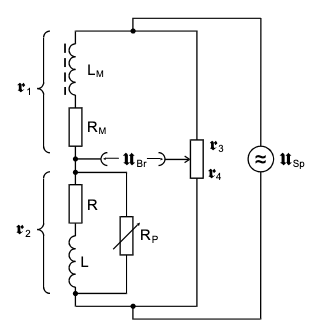
\includegraphics[width = 0.4\textwidth]{content/Bilder/Brueckenschaltung.png}
  \caption{Brückenschaltung von zwei Spulen zur Messung der Suszeptibilität \cite{anleitungV606}.}
  \label{fig:Brueckenschaltung}
\end{figure}
Je nach Messmethode wird die Suszeptibilität $\chi$ unterschiedlich bestimmt. Bei der ersten Methode wird die Brücke
abgeglichten und anschließend wird die Probe in die Zylinderspule eingeführt. Dann wird die Brückenspannung $U_{\text{Br}}$ 
gemessen. Hierbei wird die Suszeptibilität mithilfe der Knoten- und Maschenregel, sowie der Annahme, dass eine hinreichend hohe Messfrequenz verwendet wird,
bestimmt. Ebenfalls gilt $\Delta L << L$, wodurch sich 
\begin{equation}
    \chi = 4 \frac{F}{Q}\frac{U_{\text{Br}}}{U_{\text{Sp}}}
    \label{eqn:Suszeptibilität_ersteMethode}
\end{equation}
ergibt.
Bei der zweiten Methode wird zunächst die Brücke abgeglichen und nach dem Einführen der Probe wird die Brücke nochmals abgeglichen. 
Zur Bestimmung der Suszeptibilität wird die Abgleichbedingung $r_1R_4 = r_2R_3$ genutzt. Für eine kleine Abweichung $\Delta R$ und der Näherung, dass
$\Delta L << L$ gilt, lautet die Suszeptibilität
\begin{equation}
    \chi = 2 \frac{\Delta R}{R_3}\frac{F}{Q}\,.
    \label{eqn:Suszeptibilität_zweiteMethode}
\end{equation}

\subsection{Unterdrückung von Störspannungen}
Um bei der Messung der Brückenspannunge $U_{\text{Br}}$ vorhandene Störspannungen an den Ausgnagsklemmen zu vermeiden, 
wird ein Selektivverstärker eingesetz. Dieser sorgt dafür, dass die monofrequente Signalspannung blockiert wird. Die Filterkurve 
eines Selektivverstärkers ist in der Abbildung (\ref{fig:Selektivverstaerker}) abgebildet. Die Filterkurve stellt das Verhältnis von 
der Ausgangsspannung $U_{\text{A}}$ und der Eingangsspannung $U_{\text{E}}$ in Abhängigkeit von der Frequenz $\nu$ dar.
\begin{figure}[H]
    \centering
    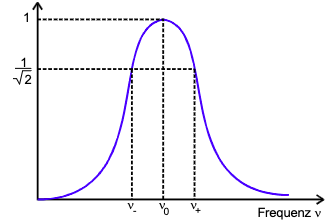
\includegraphics[width = 0.5\textwidth]{content/Bilder/Selektivverstaerker.png}
    \caption{Filterkurve eines Selektivverstärkers \cite{anleitungV606}.}
    \label{fig:Selektivverstaerker}
\end{figure} 
Die Breite der Filterkurve hängt mit der Wirksamkeit der Störspannungsunterdrückung zusammen.
Dies wird mithilfe der Güte 
\begin{equation}
    Q = \frac{\nu _0}{\nu _{+}- \nu _{-}}
    \label{eqn:Guete}
\end{equation}
beschrieben. Hier entspricht $\nu_0$ der Durchlassfrequenz und $\nu _{+}$ sowie $\nu _{-}$ sind die Frequenzen, die den Wert $\frac{U_{\text{A}}}{U_{\text{E}}} = \frac{1}{\sqrt{2}}$ besitzen. 
